\documentclass[11pt,reqno]{article}
\usepackage{amsmath,amssymb,mathrsfs,amsthm}
\usepackage[UTF8]{ctex}
%\usepackage{xeCJK}
%\setCJKmainfont{SimSum}

\usepackage{graphicx,cite,cases}
%\usepackage[pagewise]{lineno}\linenumbers
%\usepackage{refcheck}
\usepackage{xcolor}
\usepackage{bm}			% 公式加粗
\usepackage{tabularx}   % 绘制定宽表格
\usepackage{authblk}	% 添加更多作者信息
\usepackage{appendix} 	% 生成附录
\usepackage{listings}   % 附录里的代码, 支持语言高亮
\usepackage{hyperref}   % 超链接, 自动跳转
\usepackage{subfigure}  % 插入多张图片
\usepackage{tikz}
\hypersetup{hypertex=true,	% 定义超链接效果
colorlinks=true,
linkcolor=blue,
anchorcolor=blue,
citecolor=blue}

\setlength{\topmargin}{-1.5cm}
\setlength{\oddsidemargin}{0.0cm}
\setlength{\evensidemargin}{0.0cm}
\setlength{\textwidth}{16.7cm}
\setlength{\textheight}{23cm}
\headheight 20pt
\headsep    26pt
\footskip 0.4in

%%%%% 关于公式编号问题 %%%%%
%统一用equation环境
%如果需要加括号用\begin{cases}
%如果公式过长需要分行用\begin{split}
%如果一个equation里面需要多个公式, emmm没研究过

\newtheorem{theorem}{Theorem}[section]
\newtheorem{corollary}[theorem]{Corollary}
\newtheorem{lemma}[theorem]{Lemma}
\newtheorem{proposition}[theorem]{Proposition}
\newtheorem{remark}[theorem]{Remark}
\newtheorem{definition}[theorem]{Definition}
\numberwithin{equation}{section}


\renewcommand{\d}{\,\mathrm d}
\usepackage{algorithm,algorithmicx}  %写伪代码
\usepackage{algpseudocode}			% 写伪代码
%%%%%% 算法部分改为中文显示 %%%%%%%%%
%%\floatname{algorithm}{算法}
\renewcommand{\algorithmicrequire}{\textbf{Input:}}
\renewcommand{\algorithmicensure}{\textbf{Output:}}

%% Ctrl+Alt+R 编译
%% Ctrl+Alt+V 打开文档

\begin{document}

\title{微分方程数值解计算实习Lecture 6}

\author{朱荃凡}
\affil{(吉林大学数学系计算唐班)}
\date{\today}

\maketitle

\vspace{50pt}

\section{问题重述}

如图所示,\ $\Omega$表示$[0,1]^2$的区域,\ $\Gamma_1,\Gamma_2,\Gamma_3,\Gamma_4$
是它的四条边:
\begin{center}
	\begin{tikzpicture}[scale=2.5]
		% 绘制坐标轴
		\draw[->] (-0.2,0) -- (1.3,0) node[below] {$x$};
		\draw[->] (0,-0.2) -- (0,1.3) node[left] {$y$};
		% 绘制坐标轴标签
		\foreach \x in {}
			\draw (\x,0.05) -- (\x,-0.05) node[below] {$\x$};
		\foreach \y in {}
			\draw (0.05,\y) -- (-0.05,\y) node[left] {$\y$};
		% 绘制矩形
		\draw[fill=gray!20] (0,0) rectangle (1,1);
		\node[below left] at (0,0){$O$};
		\node[below] at (1,0){$(1,0)$};
		\node[left] at (0,1){$(0,1)$};
		\node[right] at (1,1){$(1,1)$};
		\node[above right] at (0.4,0.4){$\Omega$};
		\node[left] at (0,0.5){$\Gamma_1$};
		\node[right] at (1,0.5){$\Gamma_2$};
		\node[below] at (0.5,0){$\Gamma_3$};
		\node[above] at (0.5,1){$\Gamma_4$};
	\end{tikzpicture}
\end{center}
利用 Lagrange 双线性元求解区域$\Omega$区域上的偏微分问题:
\begin{equation}\label{Eqn1}
	\left\{\begin{matrix}
		-\Delta u-2\pi^2u=-2\pi^2xy,&\mathrm{in}\ \Omega,\\
		u(x,y)=0,&\mathrm{in}\ \Gamma_1,\Gamma_3,\\
	   \partial_x u(x,y)=y-\pi\sin(\pi y),&\mathrm{in}\ \Gamma_2,\\
	   \partial_y u(x,y)=x-\pi\sin(\pi x),&\mathrm{in}\ \Gamma_4.
	   \end{matrix}\right.
\end{equation}
其相应的的真解为
\begin{equation}
	u^*=xy+\sin(\pi x)\sin(\pi y).
\end{equation}

\newpage

\section{算法设计}

二维区域上的有限元问题相对一维会复杂很多,包括但不限于网格剖分,边值条件处理,积分公式.
我们分成几个部分来讨论.

\subsection{转化为变分形式}

记函数
\begin{equation}
	\begin{split}
		g_2(x,y)=y-\pi\sin(\pi y),\ &\mathrm{in}\ \Gamma_2,\\
		g_4(x,y)=x-\pi\sin(\pi x),\ &\mathrm{in}\ \Gamma_4.
	\end{split}
\end{equation}
再记函数空间
\begin{equation}
	V(\Omega)=\{v\in H^1(\Omega),\ v|_{\Gamma_1\cup\Gamma3}=0\}.
\end{equation}

那么初边值问题(\ref{Eqn1})的变分问题为:找到$u\in V(\Omega)$,使得
\[\int_\Omega\Delta u\cdot\Delta v-2\pi^2uv\d x=
\int_\Omega fv\d x+\int_{\Gamma_2}g_2v\d s+\int_{\Gamma_4}g_4v\d s,
\quad \forall v\in V(\Omega).\]

\subsection{网格剖分}

在一维有限元中,无论网格剖分的均匀与否,区间上的节点位置和其解向量中的次序是完全对应的.
这使得我们索引刚度矩阵和右端项元素时,十分容易.但是在二维有限元中,这种对应关系不存在了,
因此我们需要额外的矩阵去单独保存剖分后点,边和单元的信息.

在此问题中,我们仍使用均匀剖分.设剖分数为$N$,此时x轴和y轴均被$N$等分,\ 区域$\Omega$
上有$N^2$个小正方形单元和$(N+1)^2$个剖分节点. 下面以$N=4$为例,展示我们如何储存剖分
信息:
\begin{center}
	\begin{tikzpicture}[scale=4]
		% 绘制坐标轴
		\draw[->] (-0.1,0) -- (1.2,0) node[below] {$x$};
		\draw[->] (0,-0.1) -- (0,1.2) node[left] {$y$};
		% 绘制坐标轴标签
		\foreach \x in {}
			\draw (\x,0.05) -- (\x,-0.05) node[below] {$\x$};
		\foreach \y in {}
			\draw (0.05,\y) -- (-0.05,\y) node[left] {$\y$};
		% 绘制矩形
		\draw[fill=gray!20] (0,0) rectangle (1,1);
		% 绘制剖分
		\draw (0.25,0) -- (0.25,1);
		\draw (0.5,0) -- (0.5,1);
		\draw (0.75,0) -- (0.75,1);
		\draw(0,0.25) -- (1,0.25);
		\draw(0,0.5) -- (1,0.5);
		\draw(0,0.75) -- (1,0.75);
		% 节点编号
		\foreach \x in {0,1,2,3,4} {
    	\foreach \y in {0,1,2,3,4} {
		\pgfmathtruncatemacro{\z}{(\x)*5+\y+1} % 计算节点序号
		\pgfmathsetmacro{\xx}{\x*0.25} % 计算节点序号
		\pgfmathsetmacro{\yy}{\y*0.25} % 计算节点序号
      	\filldraw (\xx,\yy) circle (0.5pt) node[left] 
		{\footnotesize{\textit{\z}}};}}
		% 区间编号
		\foreach \x in {1,2,3,4} {
    	\foreach \y in {1,2,3,4} {
		\pgfmathtruncatemacro{\z}{\x*4-4+\y} % 计算节点序号
		\pgfmathsetmacro{\xx}{\x*0.25-0.19} % 计算节点序号
		\pgfmathsetmacro{\yy}{\y*0.25-0.175} % 计算节点序号
      	% 标记节点
      	\node[above right] at (\xx,\yy){\small{\textbf{\z}}}; }}
	\end{tikzpicture}
\end{center}

首先,将节点从下往上,从左往右依次编号,序号从1-25.对小单元也是类似的编号顺序.节点矩阵
$p$是一个$2\times25$的矩阵,其中第$i$列表示序号为$i$的节点的横纵坐标,如下所示:
\begin{equation}
	p=\begin{pmatrix}
		0& 0 & 0 & \cdots & 0.5 &0.5&0.5&\cdots& 1 & 1\\
		0& 0.25 & 0.5 & \cdots& 0.25 &0.5&0.75&\cdots& 0.75 &1
	  \end{pmatrix}.
\end{equation}
单元矩阵$t$是一个$4\times16$的矩阵,其中第$i$列表示序号为$i$的小单元,四行表示其四个
节点在$p$中的索引,如下所示:
\begin{equation}
	t=\begin{pmatrix}
		1 & 2 & 3 &\cdots& 7 & 8 &\cdots & 18 & 19\\
		2 & 3 & 4 &\cdots& 8 & 9 &\cdots & 19 & 20\\
		7 & 8 & 9 &\cdots& 13 & 14 &\cdots & 24 & 25\\
		6 & 7 & 8 &\cdots& 12 & 13 &\cdots & 23 & 24\\
		\end{pmatrix}.
\end{equation}
边矩阵$e$较为特殊,我们在处理边值条件的时候只会用到最外侧的边的信息,内部边是不需要储存的,
$e$是一个$3\times16$的矩阵,每一列代表区间边界上的一条小边,第一行和第二行是这条小边
的起点和终点在$p$中的索引.第三行表示小边属于$\Gamma_i(1\le i\le 4)$中的哪条大边,
属于$\Gamma_1$就即成$1$,属于$\Gamma_2$就即成$2$,属于$\Gamma_3$就即成$3$,
属于$\Gamma_4$就即成$4$.如下所示:
\begin{equation}
	e=\begin{pmatrix}
		1 & 2 & 3 &\cdots& 23 & 24 &1&\cdots & 15 & 20\\
		2 & 3 & 4 &\cdots& 24 & 25 &6&\cdots & 20 & 25\\
		1 & 1 & 1 &\cdots& 2 & 2 &3 &\cdots & 4 & 4\\
		\end{pmatrix}.
\end{equation}
有了剖分信息$p,t,e$以后,可以极大地简化剩余部分地编程难度.

\subsection{数值积分公式}

在此算法中,我选择了正方形区域上的九点积分公式,它是由一维高斯积分公式直接
推导出来的,以标准区间$[-1,1]\times[-1,1]$为例:
\begin{equation}
	\int_{-1}^1\int_{-1}^1f(x,y)\d x\d y
	\approx\int_{-1}^1\sum_{i=1}^{3}\omega_if(x_i,y)\d y
	\approx\sum_{i,j=1}^3\omega_i\omega_jf(x_i,y_j).
\end{equation}	
其中$x_i,y_j$为一维三点高斯积分节点$-\dfrac{\sqrt{15}}{5},0,\dfrac{\sqrt{15}}{5}.$
$w_i$为其权重$\dfrac{5}{9},\dfrac{8}{9},\dfrac{5}{9}.$易见此公式对于所有形如
$x^my^n(m,n\le 5)$的多项式都是严格取等的.本题而言中,四点高斯积分公式精度也
够,不过为了代码的通用性,还是采用了九点.


\subsection{其余部分}

\subsubsection{生成刚度矩阵和右端项}

这部分和一维有限元是比较相似的.对小单元数进行循环,计算单元刚度矩阵和局部右端项,
找到对应节点位置并更新刚度矩阵和右端项.由于每个小单元上有四个基函数,所以单元刚度
矩阵的大小是$4\times4.$由于是等距剖分,所以每个单元刚度均一致,我们可以事先算出来.

此外,这一部分我在代码的调试过程还发现了有意思的内容,但是和本次主题关系不大,因此放在
报告最后加以说明.

\subsubsection{处理边值条件}

边值条件的处理在原理上不难理解,和一维区别不大,但是在编程上难度较大.

处理Neumann边值条件时,边矩阵$e$中提供了$\Gamma_2$和$\Gamma_4$上小边的位置信息,
在此基础上我们需要像一维有限元那样去更新右端向量的数值.二维矩形区域的拉格朗日
型元在边界上仍然是线性的,计算基函数的函数值只需要做一个线性变换即可.

Dirichlet边值条件的处理过程不再赘述.

\subsubsection{画出函数图像}

在Matlab中想画出三维图像需要专门的函数surf()或者mesh().这两个函数均需要输入矩形区域
的网格节点坐标和节点处的函数值.观察画出后图像的棱角可以发现有意思的一点:Matlab在绘制此类图形时会对
网格在进行一次剖分,把每个矩形区域分成两个三角形,然后每个三角形区域上绘制一个平面即可.

\section{程序结果}
\subsection{数值解图像}
这里展示了剖分数$N=5$和$N=10$时的数值解图像,以及$N=20$时的真解图像
(显然,画真解图像也是要剖分的).
\begin{figure}[h]
	\centering
	  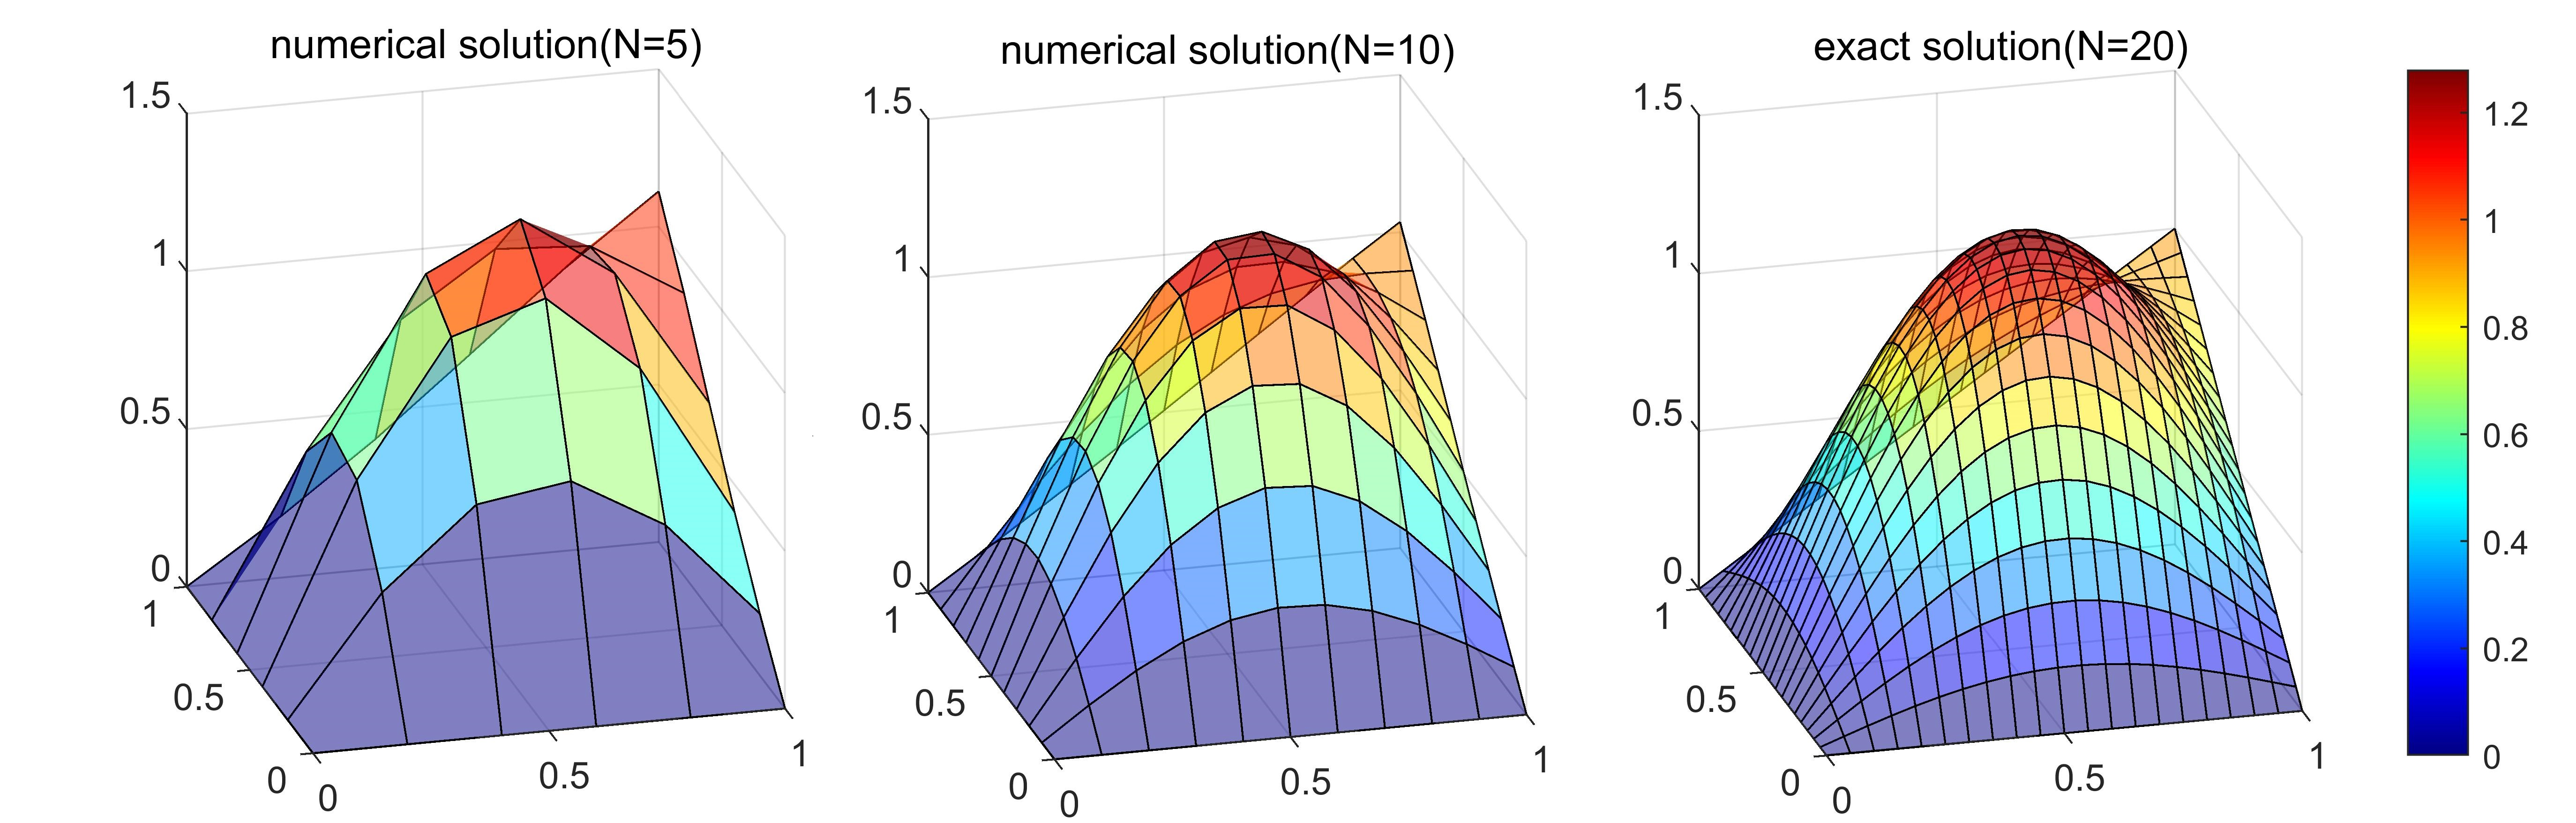
\includegraphics[width=\textwidth]{function.jpg}
	  \caption{真解和数值解}
\end{figure}

\newpage

\subsection{误差和收敛阶}
取剖分数$N=5\times2^{n-1}(1\le n\le 7),$分别计算$L^2$误差和$H^1$误差.
这里只展示了$L^2$模的误差及其收敛速度,需要注意的是横轴代表的含义是"自由度",可以
近似的认为是节点数量$(N+1)^2.$所以有些图像看起来并不均匀:
\begin{figure}[h]
	\centering
	  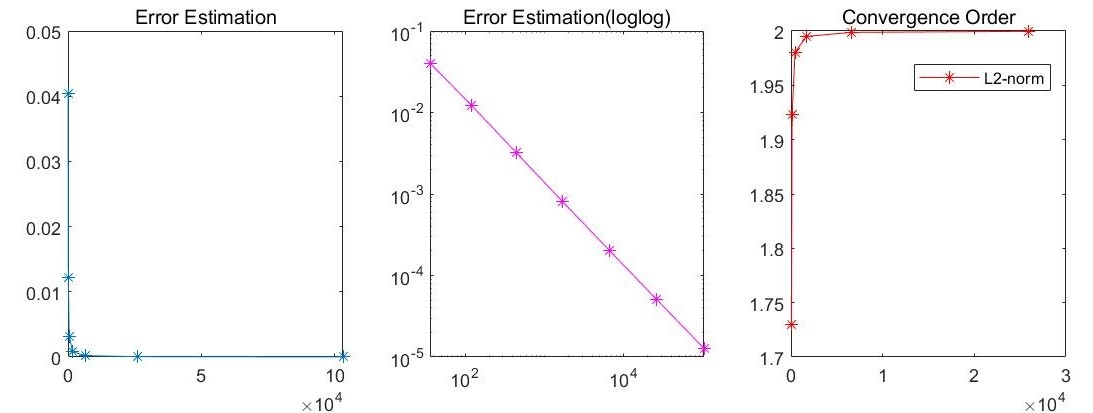
\includegraphics[width=\textwidth]{L2error.jpg}
	  \caption{$L^2$误差和收敛阶}
\end{figure}

\subsection{刚度矩阵条件数和发散阶}
剖分数如上所示,这里展示了矩阵条件数和自由度的双对数图和发散阶:
\begin{figure}[h]
	\centering
	  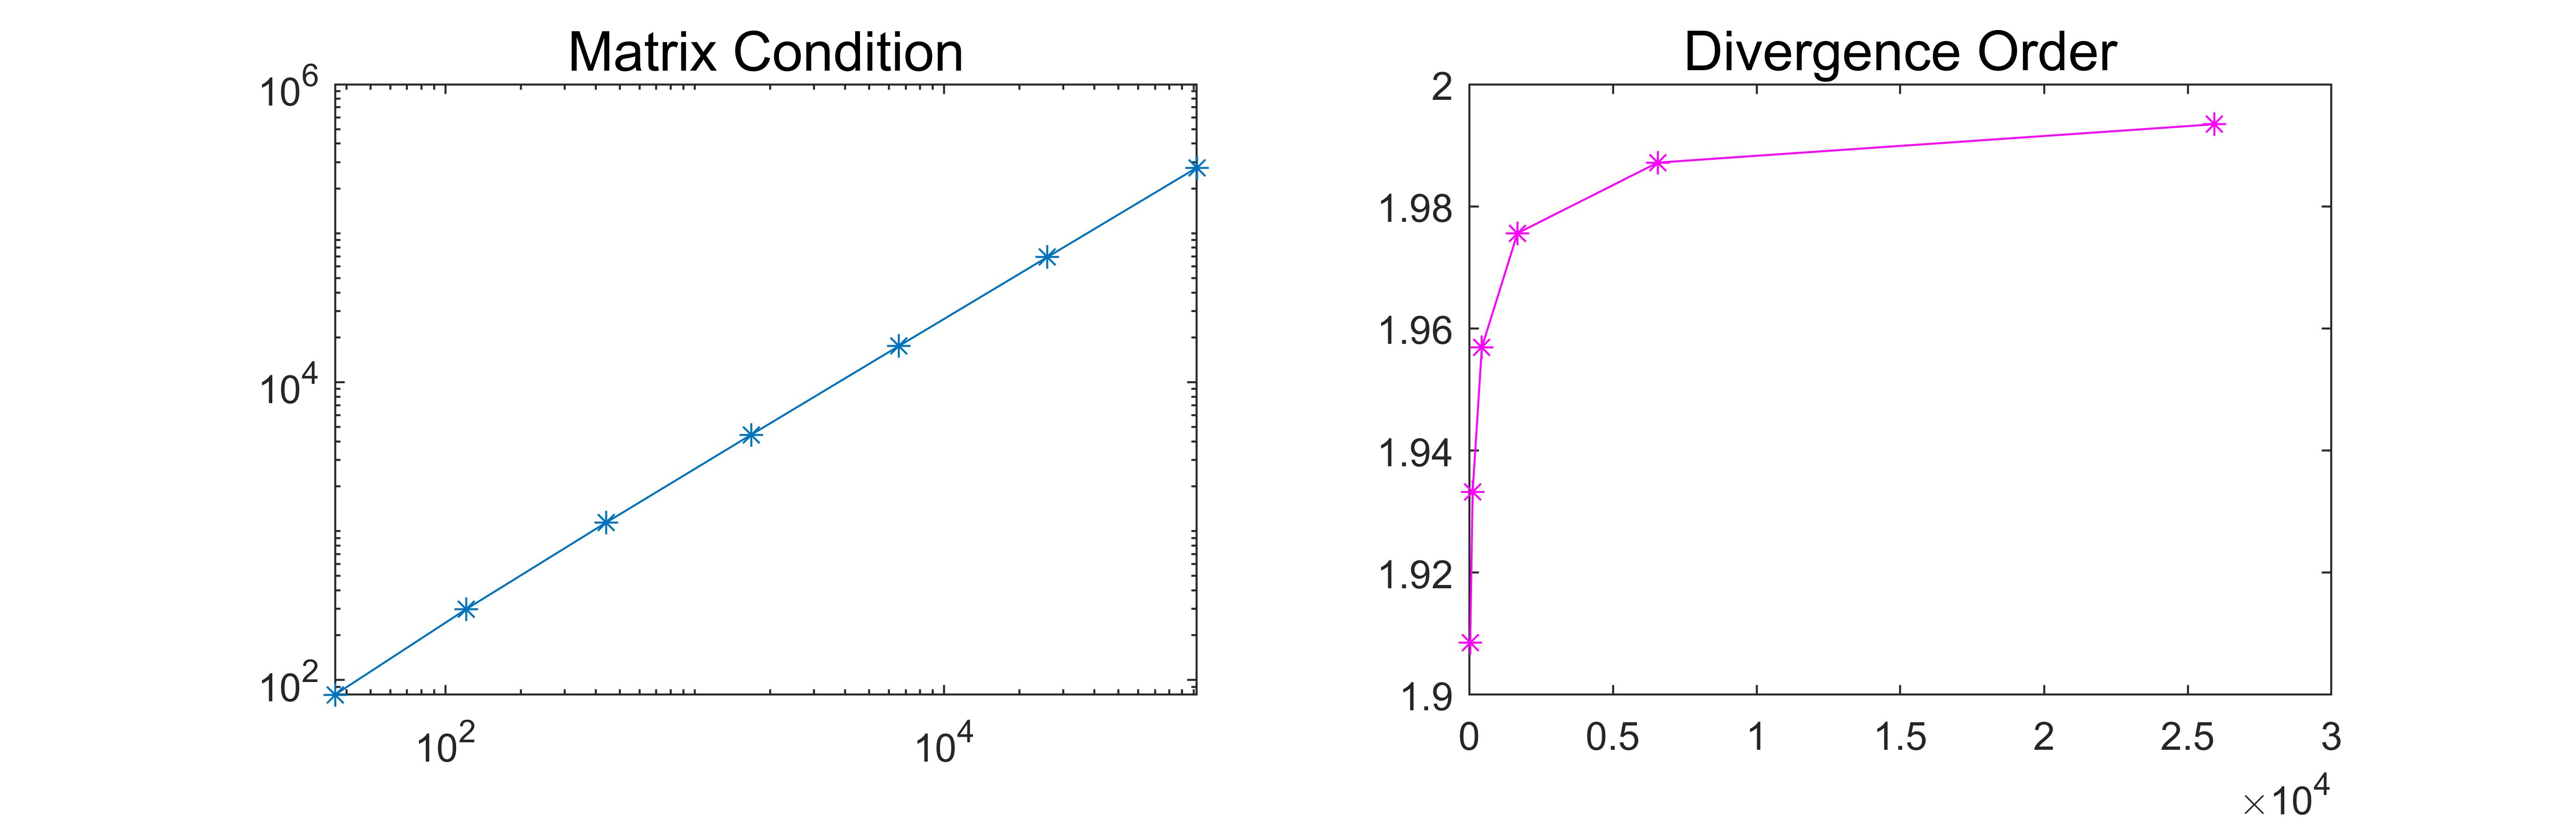
\includegraphics[width=\textwidth]{mc.jpg}
	  \caption{矩阵条件数和发散阶}
\end{figure}
有点出乎意料,发散阶仍然为二阶,这说明二阶矩形剖分后得到的线性方程组在数值计算上依旧是
相对稳定的.

\newpage
\section{关于提升运行速度的一点思考}

计算收敛阶的时候,剖分数$N=5\times2^{n-1}$是指数级增长的,节点数的增长速度就更快了.
当$n=6$时,我的程序需要算9秒,$n=7$时要算3分钟,$n=8$时,要算50分钟!

那么究竟是哪一步花了过长的时间多呢,如下是程序运行时的分析表:
\begin{figure}[h]
	\centering
	  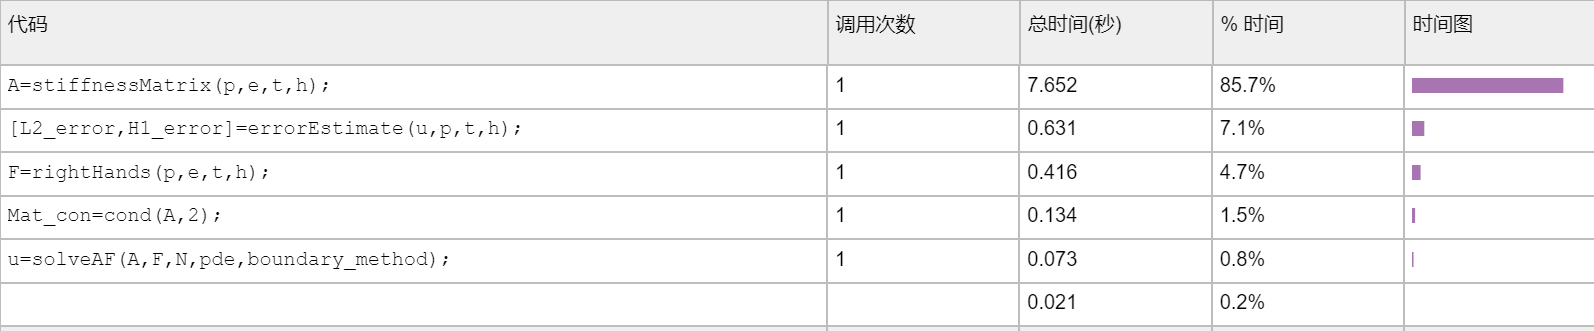
\includegraphics[width=\textwidth]{time1.png}
\end{figure}
\begin{figure}[h]
	\centering
	  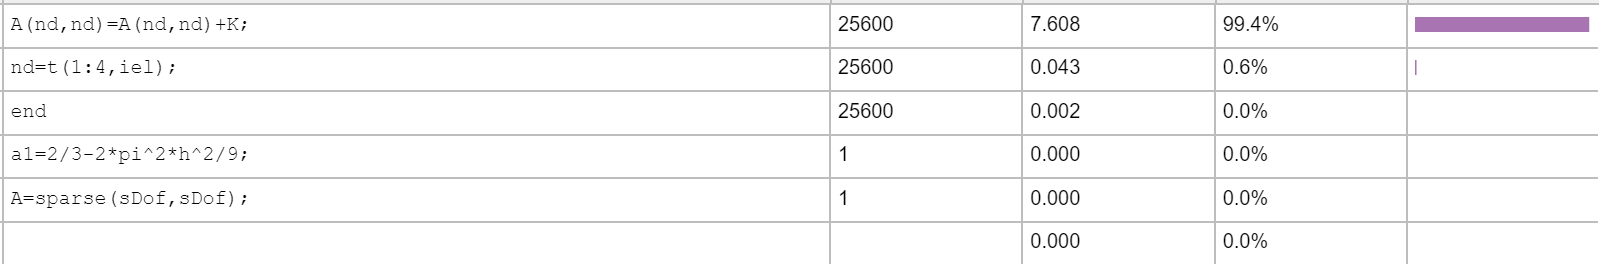
\includegraphics[width=\textwidth]{time2.png}
\end{figure}

可以看到在生成刚度矩阵,尤其是组装刚度矩阵的时候,占了格外长的时间.根据结果不难猜测是因为
生成刚度矩阵使用到了sparse()函数.好处是可以节约空间,坏处是像这样,在索引元素位置是会花费
大量的时间.

如果我们把sparse()方法改回full()方法,那么就能在3秒内跑完程序.不过需要注意,在解方程
组之前仍然需要改回稀疏矩阵,并且不能计算条件数:
\begin{figure}[h]
	\centering
	  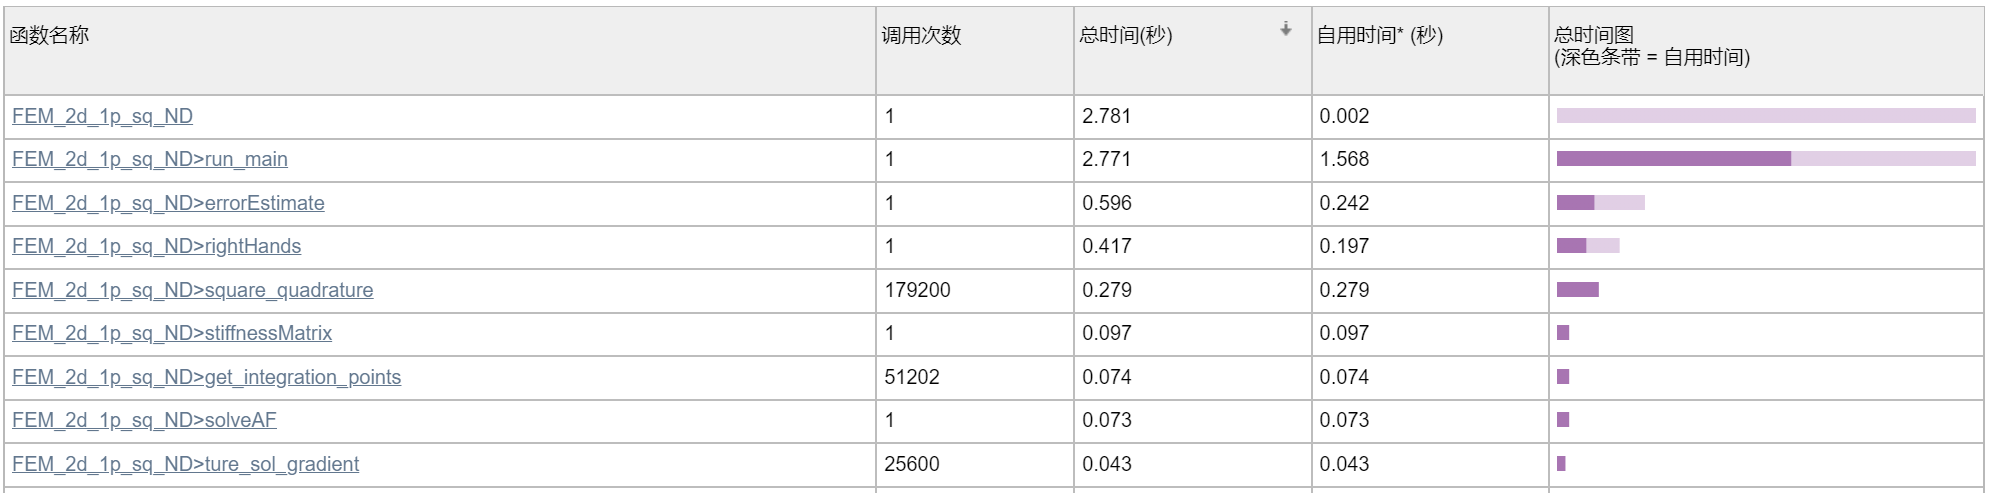
\includegraphics[width=\textwidth]{time3.png}
\end{figure}
从图中看到,生成刚度矩阵的时间被大大减少了,当时我感到很兴奋,直接就令$n=7$又算一次.

\newpage
\begin{figure}[h]
	\centering
	  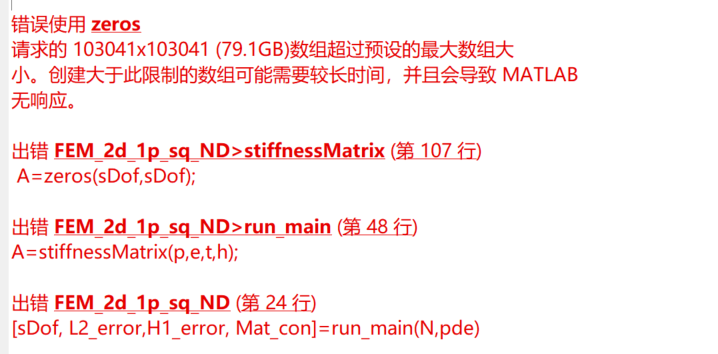
\includegraphics[width=\textwidth]{error.png}
\end{figure}
结果就得到了如上的报错----内存容量不够.所以我们可以得到结论,使用sparse()方法就是用时间换空间,使用full()方法就是用空间换
时间,在超大内存的情况可以很好的节约时间.那有没有既节约时间,又节约空间的方法呢?

答案是有的,Matlab对矩阵运算的优化很好,如果我们能把生成刚度的循环操作改成矩阵运算,
那么就能大大节约时间.我曾经在张凯老师的有限元程序里见过,40万个节点,只需要不到一分钟
就能跑完(在我程序里,n=7也才10万个节点左右).这两天我花了很多时间尝试在二维拉格朗日
型元中实现这种方法,但是做不到...
\end{document}
